\section{Methodology}

\subsection{Dataset}
Since no existing dataset for Pashto Poetry existed, we collected our dataset from scratch. A major challenge in the data collection aspect was the lack of digitalization and proper documentation on Pashto poets. While we were able to find some poetry in blogs and social sites, most of the poetry had been translated, pdf forms, or in apps for more famous poets such as Rahman Baba, Hamza Baba and Khushal Khan Khattak. In addition, poetry was also found as just a couplet or two in the form of images on social media. Thus, our data collection included searching for poetry online through blogs, articles, and sites including Hamari Web, Wordpress, and Rekhta. We also collected pdf books of poets that we passed through an OCR and then cleaned out. Since there were also mobile apps available for certain Pashto poets, we extracted from mobile apps and converted it into textual form, or took screenshots of the poetry and passed it through the OCR to get the text.

The collected data was then passed through an extensive data cleaning pipeline which involved both manual and automated cleaning. The data was first cleaned manually by removing such texts which could not be automated such as prefaces or index from books, headers or footers, authors notes, footnotes, and other such irrelevant text. Since that text was also in the same script, automating this was impossible, hence first, the data was manually inspected for such discrepencies. Then the data was passed through a data cleaning pipe where first the english characters, and other irrelevant symbols were removed including numbers, special characteres, etc, followed by removing those lines where only 1 or 2 words were present as they were mostly the titles of the poems (this was also extensively cleaned manually before), followed by removing the duplicate entries in the data, followed by removing the empty lines. Then a script would return the number of couplets in the data. The image given below describes the complete data pipeline. 

\begin{figure}[H]
    \centering
    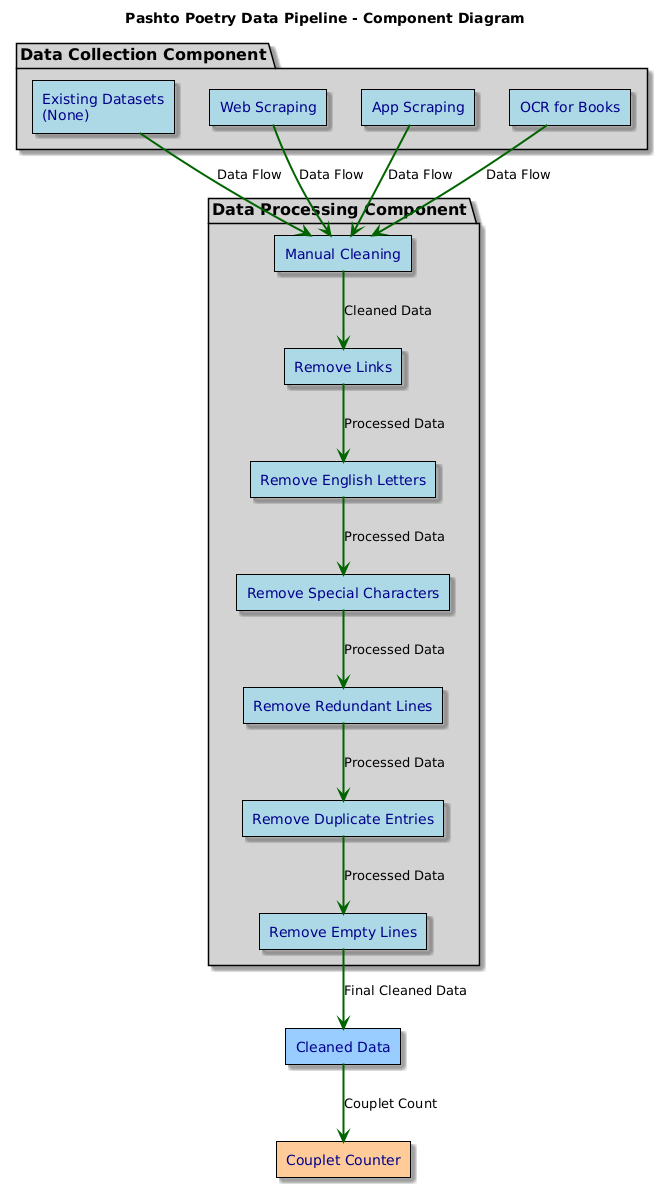
\includegraphics[width=0.35\textwidth]{datapipeline.png}
    \caption{Data Cleaning Pipeline}
    \label{fig:data-pipeline}
\end{figure}

All the data was then cleaned and sorted to get just the Pashto poetry of each poet. All in all, we were able to collect 27,607 couplets from a total of 23 poets. The chosen poets also show a good distribution in the sense that some poets are of historic ages such as Rahman Baba, Khushal Khan Khattak, and Hamza Baba, while there are also recent poets such as Ghani Khan, and Khatir Afridi. Thus, the poetry would have varying styles, themes, word usage, dialects, and vocabulary which would help in training a robust model as the patterns would be more diverse. 

The table below shows the number of couplets collected for each poet.
\begin{table}[H]
    \centering
    \begin{tabular}{|c|p{10em}|c|}
        \hline
        \rowcolor{lightgray} \textbf{No.} & \textbf{Poet/Shayari} & \textbf{Couplets Count} \\ \hline
        1. & Abbasin Yousuf & 1875 \\ \hline
        2. & Ajmal Khattak & 780 \\ \hline
        3. & Allama Abdul Hai & 2380 \\ \hline
        4. & Aziz Mazerwal & 30 \\ \hline
        5. & Ghani Khan & 1399 \\ \hline
        6. & Hamza Baba & 1177 \\ \hline
        7. & Javed Ahmedzai & 561 \\ \hline
        8. & Karan Khan & 979 \\ \hline
        9. & Khaliq Ziari & 40 \\ \hline
        10. & Khatir Afridi & 1436 \\ \hline
        11. & Khushal Khan Khattak & 4257 \\ \hline
        12. & Matiullah Turab & 1192 \\ \hline
        13. & Mumtaz Orakazi & 1645 \\ \hline
        14. & Munir Jan & 1169 \\ \hline
        15. & Naeem Ahmed & 856 \\ \hline
        16. & Rabia Mumtaz & 572 \\ \hline
        17. & Rahman Baba & 2202 \\ \hline
        18. & Rehmat Shah & 1534 \\ \hline
        19. & Sahib Shah Sabir & 1051 \\ \hline
        20. & Shabbir Khan Durrani & 1056 \\ \hline
        21. & Shakir Orakzai & 569 \\ \hline
        22. & Salim Riaz & 232 \\ \hline
        23. & Shoaib Khan Khattak & 615 \\ \hline
        \cellcolor{lightgray} \textbf{Total} & & \textbf{27,607} \\ \hline
    \end{tabular}
    \caption{Poets and their couplets count}
    \label{tab:poets-couplets-table}
\end{table}

The histogram below shows the distribution of the poets in the dataset.
\begin{figure}[H]
    \centering
    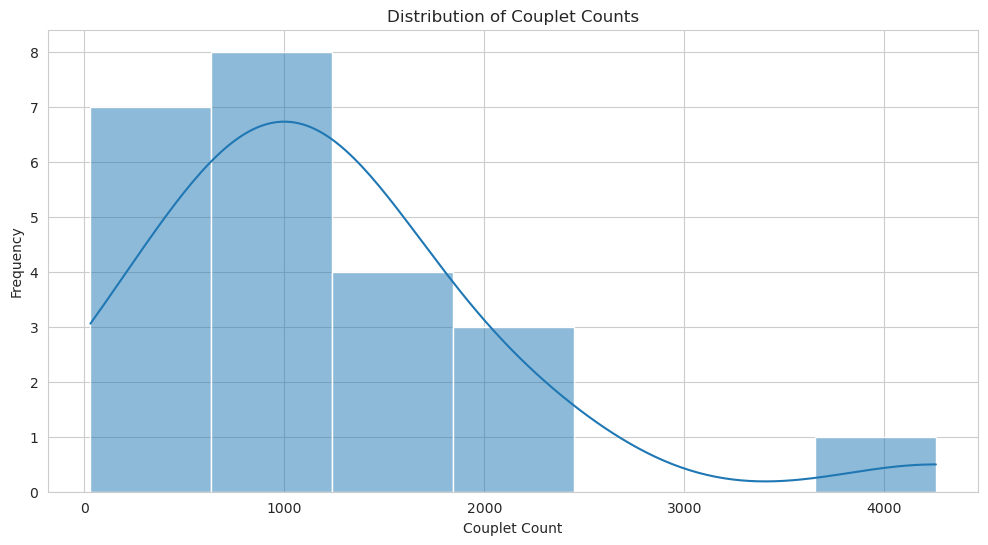
\includegraphics[width=0.475\textwidth]{poet_dist_hist.png}
    \caption{Poet Distribution}
    \label{fig:poet-dist-hist}
\end{figure}
It shows that the dataset is imbalanced, with some poets having a very high number of couplets, while some poets have a very low number of couplets. This imbalance in the dataset could lead to the models overfitting on the poets with a high number of couplets, and not learning the features of the poets with a low number of couplets well enough.

We also decided to remove 3 of the poets for our models with the lowest poet count - mainly Aziz Mazerwal, Khaliq Ziari, and Salim Riaz. The final dataset that we trained our models on consisted of 20 poets then. 

\subsection{Machine Learning Models}
From our extensive literature review, we found that machine learning models have been widely used for classification and attribution tasks. Thus, we decided to employ several machine learning models to classify Pashto poetry. Our main machine learning pipeline includes first label encoding the dataset, followed by extracting features from the text data based on TF-IDF Feature Extraction. TF-IDF Feature Extraction works by first tokenizing the text data, followed by converting the text data into a matrix of token counts, and then normalizing the token counts. The TF-IDF value increases proportionally to the number of times a word appears in the document but is offset by the frequency of the word in the corpus. This helps in reducing the importance of common words in the text data. For our models, we extracted 10000 features. The TF-IDF vectors were then split into 80-20 train-test split. Since our dataset was heavily imbalanced, we decided to go for a weighted train-test split, where the train-test split was done in such a way that the distribution of the classes in the train and test set was the same, thus, each class had the same ratio of samples in the train and test set. Finally, those TF-IDF vectors were then passed through several machine learning models including Random Forest, Support Vector Machine, Logistic Regression, and XGBoost, as they all were supported by the literature. The diagram below explains the complete machine learning pipeline.

\begin{figure}[H]
    \centering
    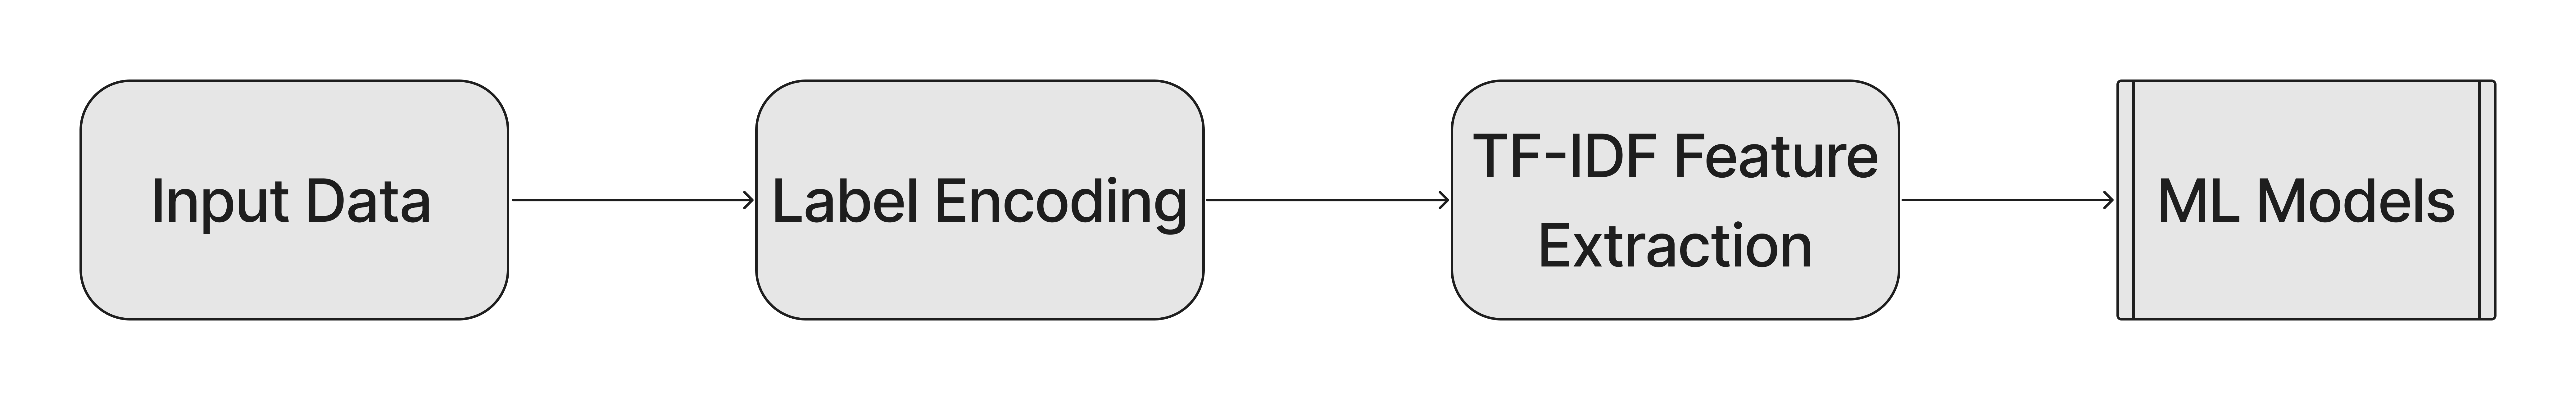
\includegraphics[width=0.45\textwidth]{ml_pipe.png}
    \caption{Machine Learning Pipeline}
\end{figure}

We used python's ``Pandas'' library for creating the dataframes, and for labelling the data for the 20 poets. We defined our own weighted train-test split function to ensure that the distribution of the classes in the train and test set was the same. Python's ``TfidfVectorizer'' was used for the TF-IDF feature extraction. Lastly, we used the ``Scikit-learn'' library for the machine learning models, and the ``XGBoost'' library for the XGBoost model.

\subsubsection{Random Forest}
Random Forest is an ensemble learning method that operates by constructing a multitude of decision trees at training time and outputting the class that is the mode of the classes of the individual trees. Random Forest is a bagging technique and is an ensemble of decision trees. We trained our Random Forest model on 100 esimators, with no max-depth defined. We tried hyperparameter tuning of the Random Forest model as well with various parameters, however, they did not improve the model performance. 

\subsubsection{Support Vector Machine}
Support Vector Machine is a supervised machine learning algorithm that can be used for both classification or regression challenges. From the literature, we found that SVM has been widely used for text classification tasks. We experimented with the linear kernel, rbr kernel with gamma set to scale and C set to 1 as this was the best performing hyperparameters for our dataset.

\subsubsection{Logistic Regression}
Logistic Regression is a statistical model that in its basic form uses a logistic function to model a binary dependent variable. We used the Logistic Regression model on 1000 iterations, we also implemented a liblinear solver, and a newton-cg solver with a C value of 10. 

\subsubsection{XGBoost}
XGBoost is an optimized distributed gradient boosting library designed to be highly efficient, flexible, and portable. It implements machine learning algorithms under the Gradient Boosting framework. We used the XGBoost model with 100 n estimators, a max depth of 3, a learning rate of 0.1, gamma set to 0.1, eval metric set to logloss, and a scale pos weight of 1, as this was the best performing hyperparameters for our dataset.


\subsection{Deep Learning Models}
We also experimented with deep learning models for Pashto poetry classification. Deep Learning models are inspired by the structure and function of the brain, in which the neural networks work in a similar way to the human brain, updating and learning their weights and biases based on the input data. As such, deep learning models have been quite powerful, and robust in their ability to learn complex patterns in the data. Therefore, they have also been widely used for text classification tasks.  

We used the Keras library with TensorFlow backend for our deep learning models. Our deep learning pipeline included first labelling and one-hot encoding the input data, followed by tokenizing the text data, and then padding the text data to a fixed length. We then used an embedding layer to convert the text data into a dense vector of fixed size. Those embeddings were then passed through our deep learning models. The figure below illustrates the complete deep learning pipeline.

\begin{figure}[H]
    \centering
    
\includegraphics[width=0.45\textwidth]{dl_pipe.png}
    \caption{Deep Learning Pipeline}
\end{figure}

We used the ``Pandas'' library for creating the dataframes. The ``Label Encoder'' was used for label encoding the 20 poets in our dataframes. We used our previous weighted train-test split function for splitting the data into train, validation and test sets. We used an 75-5-20 train-validation-test split. The remaining methodology remains the same for tokenization, padding, and embedding layers. We used the ``Keras'' library for the deep learning models, and the ``TensorFlow'' library for the backend.

We initially thought of using Bi-LSTM, Bi-GRU, and CNN models for our deep learning pipeline. However, after various experimentation and hyperparameter tuning, we found that those deep learning models were not performing well on our dataset, mostly overfitting on the training data due to which we were not getting a desired validation or test accuracy as expected. Therefore, after experimenting with the Bi-LSTM model, we decided to move onto other Deep Learning models instead. 

\subsubsection{Bi-LSTM}
For the Bi-LSTM model, we used 3 Bi-LSTM layers with 64, 32, and 16 units respectively. We also used a dropout layer with a dropout rate of 0.3 after each Bi-LSTM layer. We used the softmax activation function for the output layer. We used the Adam optimizer with a learning rate of 0.001, and sparse categorical cross-entropy as the loss function. We used early stopping with a patience of 10 epochs. We trained the model for 20 epochs with a batch size of 32. We also experimented with various hyperparameters for the Bi-LSTM model, including the number of units, the number of layers, the dropout rate, the learning rate, and the batch size. We also implemented a simple LSTM model, however, the Bi-LSTM model performed better than the simple LSTM model, but even that was overfitting on the training data. We suspect the overfitting was due to the small dataset size, and similar features in the poetry of different poets. Therefore, we decided not to move on with more traditional deep learning models and instead move on to transformer models instead.


\subsection{Transformer Models}

Tranformers are a type of deep learning model aimed at solving natural language processing, and other sequence-based tasks such as text classification, generation, and translation. Transformers have been widely used for text classification tasks due to their ability to learn long-range dependencies in the data. They utilize the power of attention, and encoder decoder architecture. As from our literature review, transformer based models can be seen to perform well in the recent papers for text classification tasks, we decided to experiment with transformer models for Pashto poetry classification. We experimented with a few transformer based models; DistilBERT, Bert based Multilingual Uncased, Meta Llama3.2-1B, Mt5 Multilingual XLSum, and Mt0 Base.

The methodology remains the same as for the Deep Learning models, since transformers are essentially deep learning models. We used the ``Pandas'' library for creating the dataframes. The ``Label Encoder'' was used for label encoding the 20 poets in our dataframes. We used our previous weighted train-test split function for splitting the data into train, validation and test sets. We used an 80-10-10 train-validation-test split. The remaining methodology remains the same for tokenization, padding, and embedding layers where needed. We used the ``Hugging Face'' library for the transformer models, and the ``TensorFlow'' library for the backend. 


% \subsubsection{roBERTa}
% roBERTa is a robustly optimized BERT approach, which is a transformer-based model. It is a variant of BERT, and has been pre-trained on a large corpus of text data. We used the ``Hugging Face'' library for the roBERTa model.


\subsubsection{DistilBERT}
DistilBERT is a distilled version of BERT, which is a transformer-based model. It is a smaller version of BERT, and has been pre-trained on a large corpus of text data. We used the ``Hugging Face'' library for the DistilBERT model. 


\subsubsection{Meta Llama}
We used the Meta Llama 3.2 model, which is collection of multilingual large language models (LLMs) is a collection of pretrained and instruction-tuned generative models in 1B (billion parameters) and 3B (billion parameters) sizes (text in/text out). The Llama 3.2 instruction-tuned text only models are optimized for multilingual dialogue use cases, including agentic retrieval and summarization tasks. They outperform many of the available open source and closed chat models on common industry benchmarks. For our task, we opted for the 1B model. We used the ``Hugging Face'' library for the Meta Llama model. 

\subsubsection{Bert Based Multilingual Uncased}
We also tried the Bert Based Multilingual Uncased model, a pretrained model of 168M (million) parameters, on the top 102 languages with the largest Wikipedia using a masked language modeling (MLM) objective. The MLM model takes a sentence, and randomly masks 15\% of the words in the input then run the entire masked sentence through the model and has to predict the masked words. This is different from traditional recurrent neural networks (RNNs) that usually see the words one after the other, or from autoregressive models like GPT which internally mask the future tokens. It allows the model to learn a bidirectional representation of the sentence. We used the ``Hugging Face'' library for the Bert Based Multilingual Uncased model.

\subsubsection{Mt5 Multilingual XLSum} 
The Mt5 Multilingual XLSum is based on Google's Mt5 model, which is a checkpoint finetuned on the 45 languages of the \href{https://huggingface.co/datasets/csebuetnlp/xlsum}{XLSum Dataset}, which includes Pashto as well. 

\subsubsection{Mt0 Base}
We also trained the Mt0 Base model by bigscience, based on BLOOMZ and mT0, a family of models capable of following human instructions in dozens of languages zero-shot. They fintuned BLOOM and mt5 pretrained multilingual models on their crosslingual task mixture (xP3), and found that their resulting model was capable of crosslingual generalization to unseen tasks and languages. Their model is finetuned on 101 languages, including Pashto, hence we decided to experiment with this model as well.